\documentclass[10pt,xcolor=pdflatex]{beamer}
\usepackage{newcent}
\usepackage[utf8]{inputenc}
%\usepackage[czech]{babel}
\usepackage{hyperref}
\usepackage{fancyvrb}
\usetheme{FIT}

%%%%%%%%%%%%%%%%%%%%%%%%%%%%%%%%%%%%%%%%%%%%%%%%%%%%%%%%%%%%%%%%%%
\title[]{Counting People Using a PIR Sensor}

\author[]{Martin Beneš}

\institute[]{Brno University of Technology, Faculty of Information Technology\\
Božetěchova 1/2. 612 66 Brno - Královo Pole\\
xbenes49@stud.fit.vutbr.cz}

%\date{January 1, 2016}
\date{\today}
%\date{} % bez data

%%%%%%%%%%%%%%%%%%%%%%%%%%%%%%%%%%%%%%%%%%%%%%%%%%%%%%%%%%%%%%%%%%

\begin{document}

\frame[plain]{\titlepage}


% ---- AIM ---- %
\begin{frame}\frametitle{The aim}
    \begin{itemize}
        \item Study the topic.
        \item Design a theoretical system, that could:
            \begin{itemize}
                \item \emph{Localize} a person.
                \item Estimate \emph{a count} of people.
            \end{itemize}
        \item Implement and test the approach.
        \item Summarize.
    \end{itemize}
\end{frame}

% ---- DESIGN ---- %
\begin{frame}\frametitle{The design}
    \begin{itemize}
        \item Sensor device
            \begin{itemize}
                \item PIR STD
                \item NodeMCU (C++/Arduino)
            \end{itemize}
        \item Classification server
    \end{itemize}

    \begin{center}
        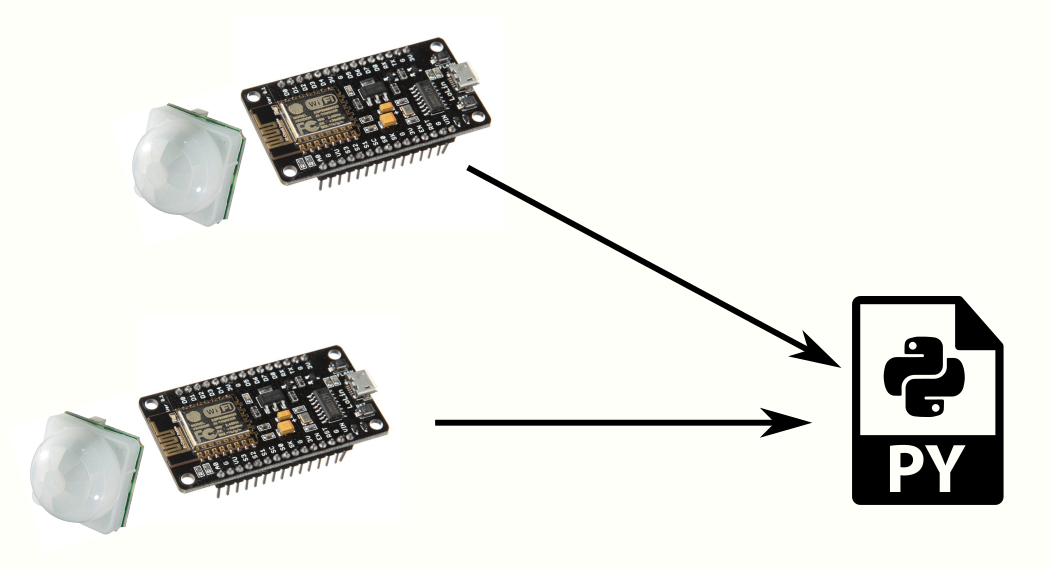
\includegraphics[width=0.7\textwidth]{img/structure.png}
    \end{center}
\end{frame}

% ---- PROGRAM ---- %
\begin{frame}\frametitle{Classification}
    \begin{center}
        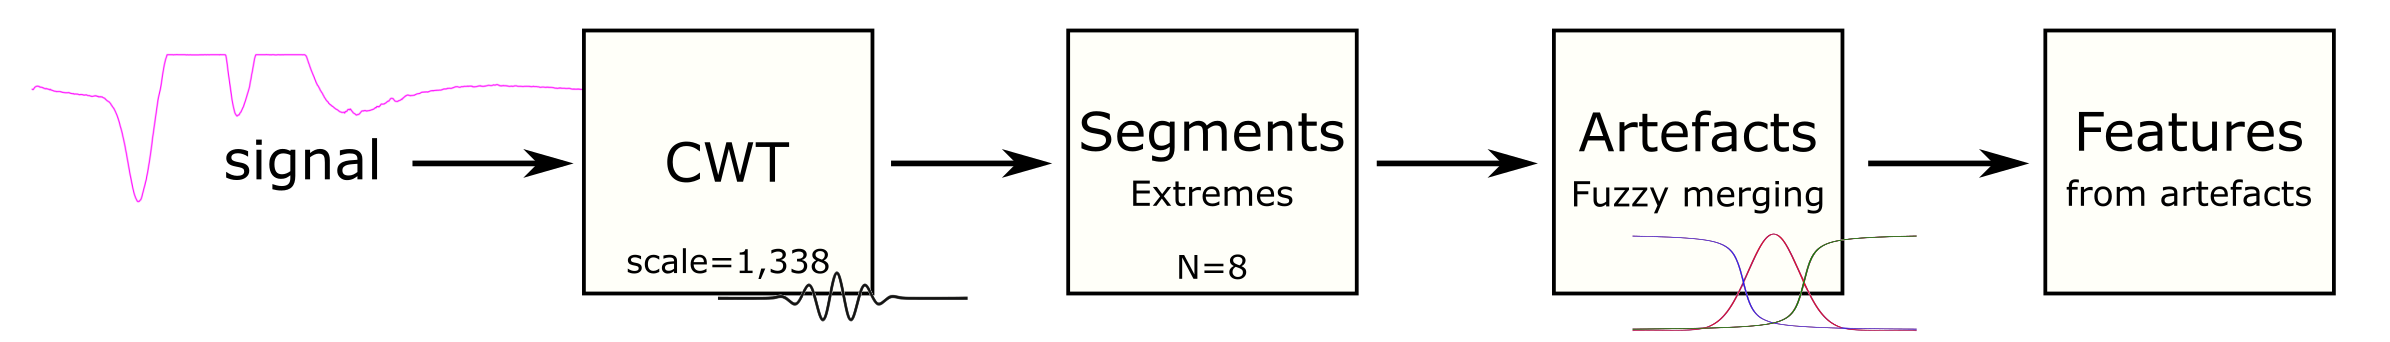
\includegraphics[width=1\textwidth]{img/features.png}
    \end{center}
\end{frame}


% ---- END ---- %
\bluepage{Thank You For Your Attention !}

\end{document}
